\chapter{Project Plan}\label{ch:style}

\section{Minimum Viable Product (MVP)}

    \begin{wrapfigure}{r}{0.55\textwidth}
        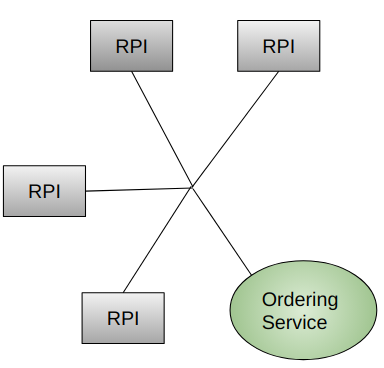
\includegraphics[width=0.9\linewidth]{network.png} 
        \caption{Raspberry Pi Network}
        \label{fig:wrapfig}
    \end{wrapfigure}
    
    For the MVP, the goal is to run Hyperledger Fabric, with four organisations participating in the network. The network will consist of four Raspberry Pi's and one computer. The Raspberry Pi's will run the peer nodes of HLF, each of which will belong to one organisation in the consortium, while the computer will run a node participating as an ordering node, forming the ordering service. The ordering node will be owned by one of the participating organisation.
    
    We want the network to perform basic operations such as transactions that allow for change of ownership. An example run through of the transactions we want to perform, is: 
    
    
    First provide one of the organisations with ownership of an item in the ledger, we will then perform transactions which transfer the item through the four participating organisations. This is considered the minimum required run through for the network.
    
    The peer nodes in the network will each hold copies of the ledger and smart contracts that will be used to perform transactions on the network. 
    
    The ordering node will be run on a computer, which does not face the same limitations of the Raspberry Pi's due to the in real world use cases of HLF, the ordering service can be run off site from the rest of the network, with only the devices running peer nodes required to be on site. The Raspberry Pi's used for the implementation will preferably be Raspberry Pi 4 Model B's, but depending on availability Raspberry Pi 3 Model B's may be used. The computer used will be a commercial laptop.
    
\section{Further Stages}

    \subsection{Testing Suite}
    Following the MVP, the next step is to implement the testing suite. This will likely be implemented in JavaScript(JS), the reasoning being that HLC has been implemented in JS, allowing for easier reference when building our own implementation. 
    
    We will first attempt to implement the node specific testing such as CPU consumption, followed by the blockchain network testing. This is due to the need to understand at what point the Raspberry Pi's may fail under load from running HLF.
    
    \subsection{Improving the Network}
    After the testing suite has been implemented, improving the network will be the next step, this will involve improving smart contract functionality. One idea is to add a sensor, such as a temperature sensor, to one of the Raspberry Pi's and periodically commit readings to the ledger. Then having smart contracts on the ledger that monitor the committed readings, and if they are outside of a certain range it raises a warning and/or commits some form of notification . This is considered as it may be a functionality that an industry, like supply chains, require.
    
    \subsection{Ordering Service}
    If all other sections are finished, then porting the ordering node off of the computer onto a Raspberry Pi will be attempted. While it is not considered necessary to run an ordering node on a Raspberry Pi, it would serve to further the proof of concept of how a consortium blockchain could run on a IoT network.
    
    
    
    
    
\section{Required Skills}

In order to achieve the goals of this thesis, there is the need to learn and practice several skills.
The ability to run and manage a HLF fabric network is the first major skill that will need to be learnt as it forms the backbone of the thesis. This will be learnt through the documentation provided by The Hyperledger Foundation, which is extensive and readily accessible. A part of learning HLF, involves learning and implementing smart contracts  HLF supports smart contracts written in Go, JS and Java, due to stronger past experience in using JS over the other languages, this is the language that will be chosen to create and run our smart contracts.

To be able to run HLF on the network of Raspberry Pis, upskilling in using IoT devices will also be required. In order to manage the multiple devices and their nodes, using a technology like Docker Swarm will be required. Further understanding of the limitations of Raspberry Pis and how to deal with these challenges will also be necessary.
https://www.overleaf.com/download/project/5f2a624fb4e0910001deca32/build/175e31aad5a-194f9c2fd379452c/output/output.pdf?compileGroup=standard&clsiserverid=clsi-pre-emp-e2-a-l3g9&popupDownload=true
The testing suite will also require a new set of skills, with the intention of implementing in JS, learning how to implement testing suites in JS will be required, this is expected to not have much overlap with the JS involved learnt for smart contracts in HLF, as such it is expected to require significant amounts of time 

\section{Thesis Timeline}

    \begin{figure}[!htb]
        \centering
        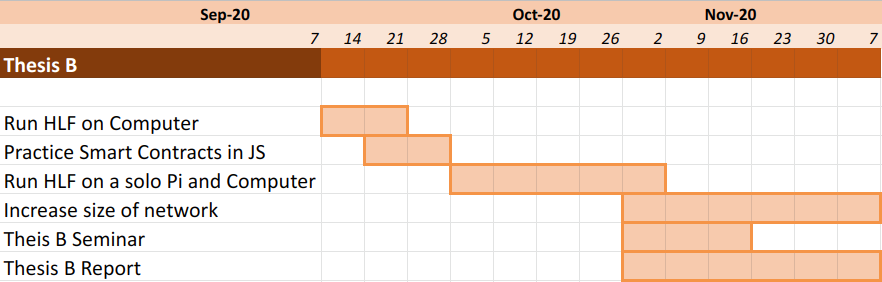
\includegraphics[width=\columnwidth]{images/termB.png}
        \caption{Thesis B Plan}
        \label{fig:my_label}
    \end{figure}
    
    \begin{figure}[!htb]
        \centering
        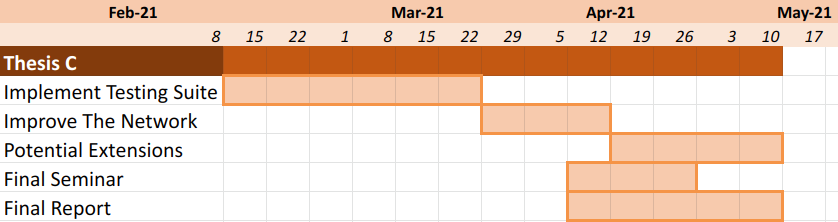
\includegraphics[width=\columnwidth]{images/C Plan.png}
        \caption{Thesis C Plan}
        \label{fig:my_label}
    \end{figure}
    
 
    The table allocates time for each section in the weeks available per term. The timeline determined the ordering of each part due to requirement of learning how to interact with each part, such as learning how to run HLF on a computer first before attempting to implement HLF on a network of Raspberry Pi's.
    
    Before a blockchain network on multiple Pi's is able to be implemented, running HLF on a single Raspberry Pi with a computer running the more intensive parts will need to be completed first. Following this, the MVP will be attempted, where more Raspberry Pis will be added into the network.
    
    The testing suite requires the implementation of the MVP. The MVP is estimated to need 6 weeks of thesis B, as such the testing suite is not expected to be started until thesis C. The testing suite is also estimated to take a total of 6 weeks of thesis C, including upskilling and implementation.
  
% \section{}
% Methodology and approach
% - Decompose the whole project into multiple
% components
% - Explain the functions of each component and
% how you would tackle each component
% • Thesis timeline – for next two terms (term for
% those doing both Thesis A and Thesis B in one
% term)
% • Justification of time allocation for each
% component
% • Required training and upskilling identified